\chapter{Supplementary Visualizations}

\begin{figure}[htbp]
    \centering
    \rotatebox{-90}{
        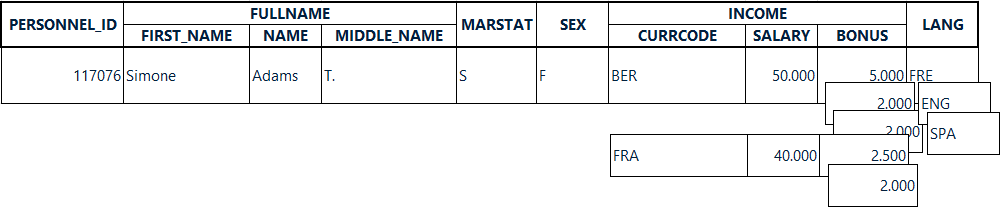
\includegraphics[width=1.2\textwidth]{chapters/images/datastructures.png}
    }
    \caption{Example structure of a record containing various Adabas data structures (enlarged)}
    \label{fig:appendix02:adabasstructure}
\end{figure}

\begin{figure}[htbp]
 \centering
 \rotatebox{-90}{
        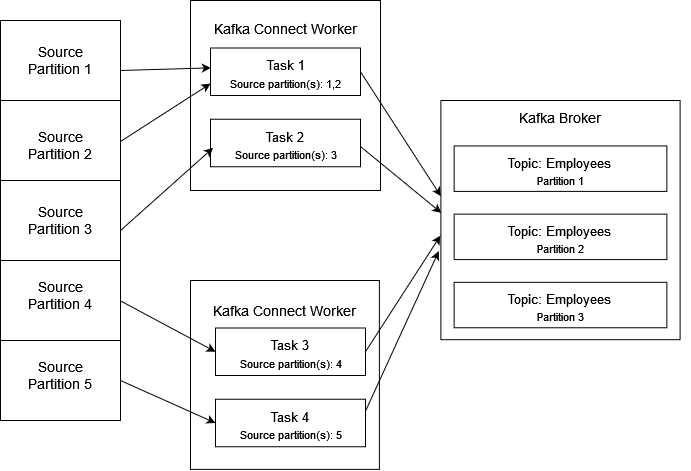
\includegraphics[width=1.2\textwidth]{chapters/images/kafka connect architecture enlarged.drawio.png}
    }
 \caption{Example Architecture of a Kafka Source Connector in Distributed Mode (enlarged)}
 \label{fig:appendix02:kafkaconnectarchitecture}
\end{figure}

\begin{figure}[htbp]
 \centering
 \rotatebox{-90}{
     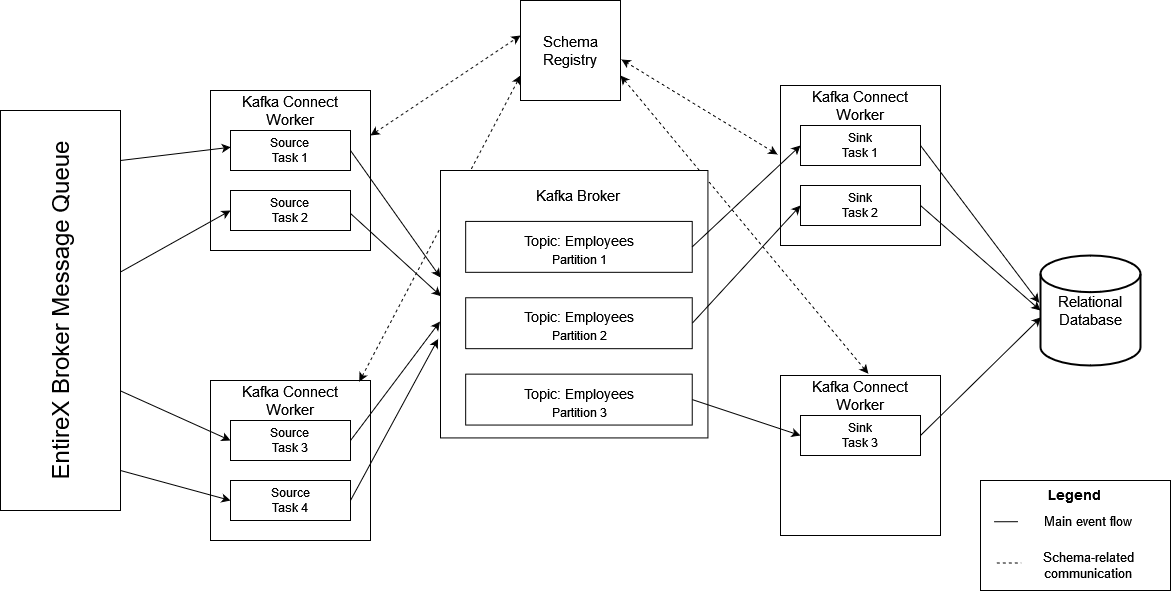
\includegraphics[width=1.6\textwidth]{chapters/images/kafka pipeline overall architecture enlarged.drawio.png}
 }
 \caption{Overall architecture of Kafka replication pipeline (enlarged)}
 \label{fig:appendix02:overallarchitecture}
\end{figure}

\begin{figure}[htbp]
 \centering
 \rotatebox{-90}{
    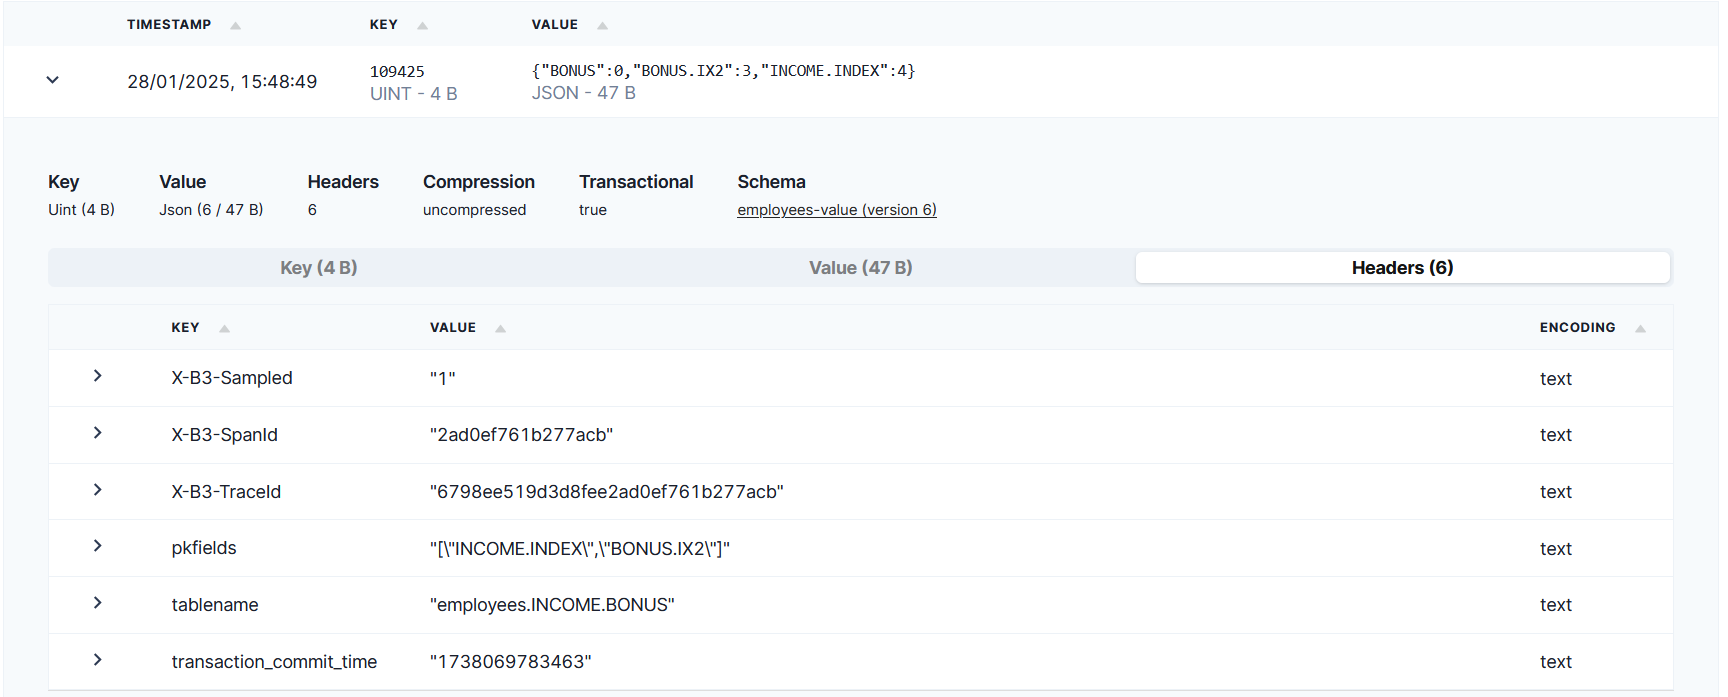
\includegraphics[width=1.7\textwidth]{chapters/images/header-example.png}
 }
 \caption{Kafka Message with header shown (enlarged)}
 \label{fig:appendix02:implementation:headerexample}
\end{figure}

\begin{figure}[htbp]
 \centering
 \rotatebox{-90}{
    \includegraphics[width=1.4\textwidth]{chapters/images/kafka prometheus monitoring stack enlarged.drawio.png}
 }
 \caption{Monitoring Stack with Prometheus and Grafana (enlarged)}
 \label{fig:appendix02:metrics:prometheusstack}
\end{figure}

\centering
\begin{figure}[htbp]
    \centering
    \rotatebox{-90} {
        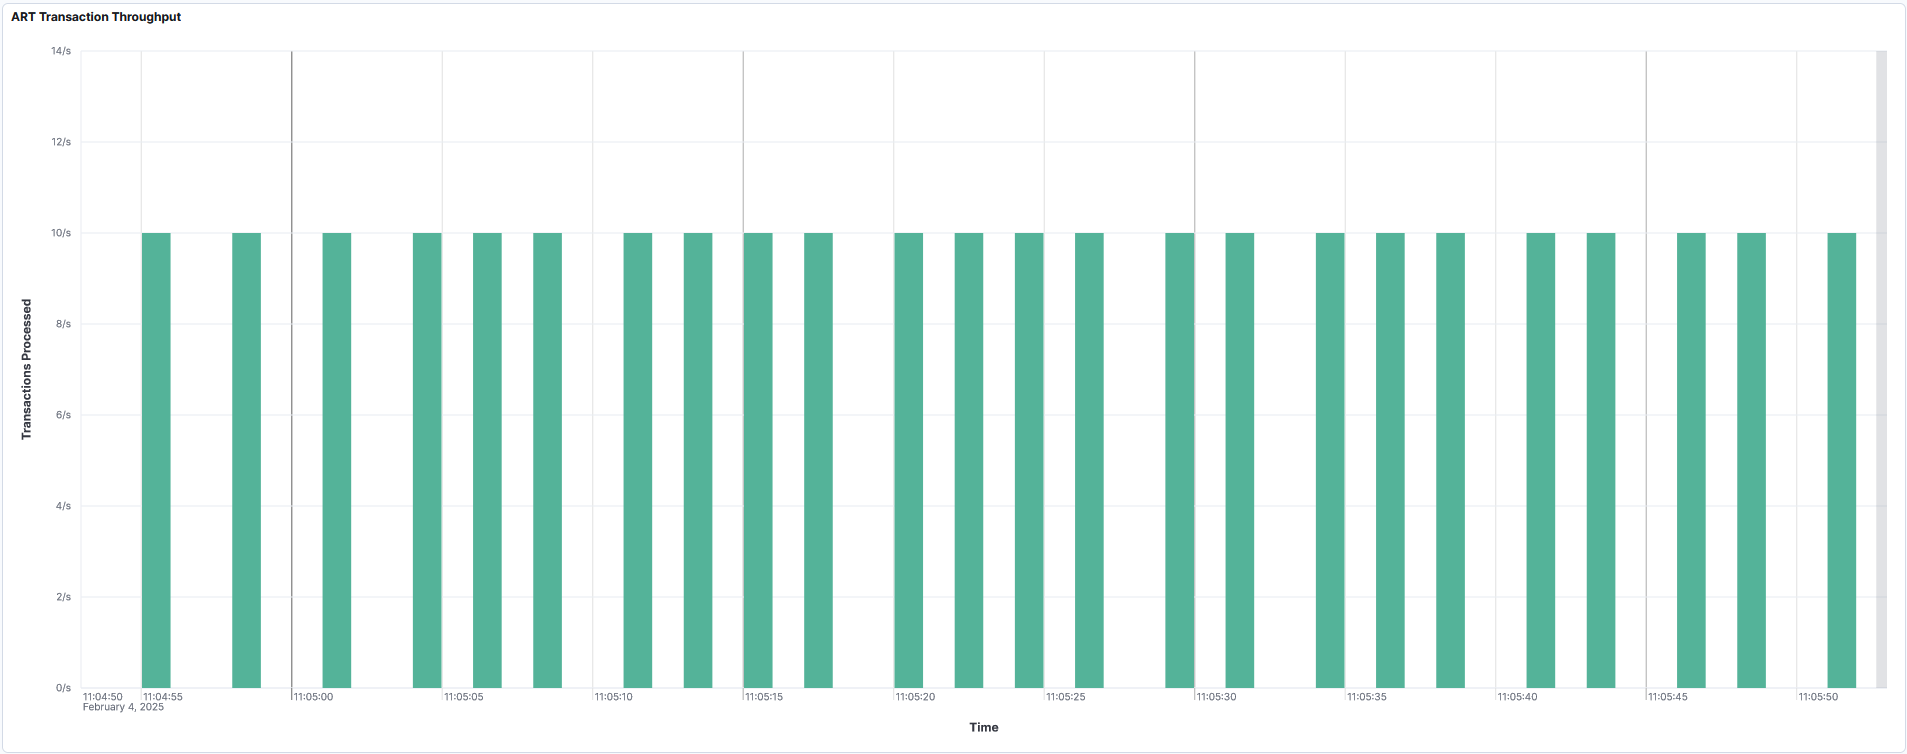
\includegraphics[width=1.8\textwidth]{chapters/images/art-performance/art-transaction-throughput-minute.png}
    }
    \caption{Metric collection excerpt of Target Adapter's processed transactions (enlarged)}
    \label{fig:appendix02:results:arttransactionminute}
\end{figure}
%%%%%%%%%%%%%%%%%%%%%%%--------MESSAGE THROUGHPUT SOURCE--------%%%%%%%%%%%%%%%%%%%%%%%%
\begin{figure}[htbp]
    % \centering
    \subfloat[Scenario 1]{\label{fig:appendix02:results:sourcemessages:scenario1}
        % \centering
        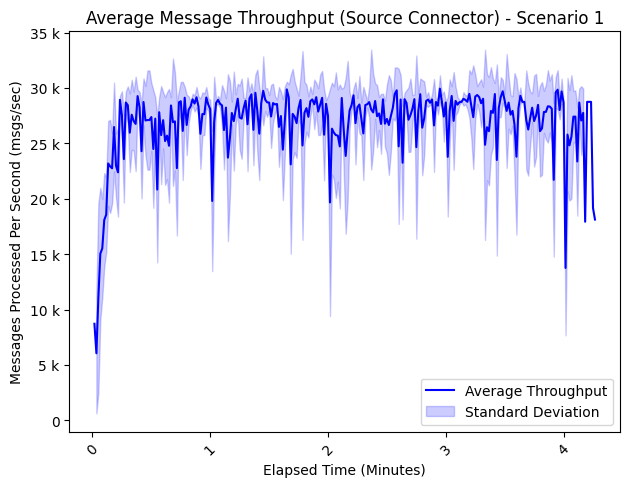
\includegraphics[width=0.5\textwidth]{chapters/images/source-performance/source-avg-messages-scenario1.png}
    }
    % \hfill
    \subfloat[Scenario 2]{\label{fig:appendix02:results:sourcemessages:scenario2}
        % \centering
        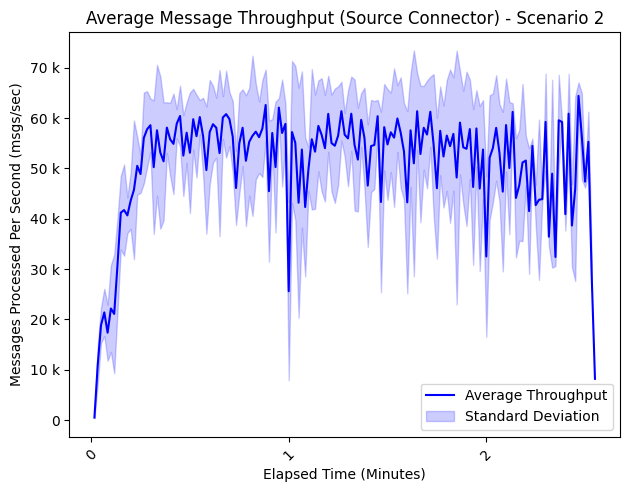
\includegraphics[width=0.5\textwidth]{chapters/images/source-performance/source-avg-messages-scenario2.png}
    }
    \hfill
    \subfloat[Scenario 3]{\label{fig:appendix02:results:sourcemessages:scenario3}
        % \centering
        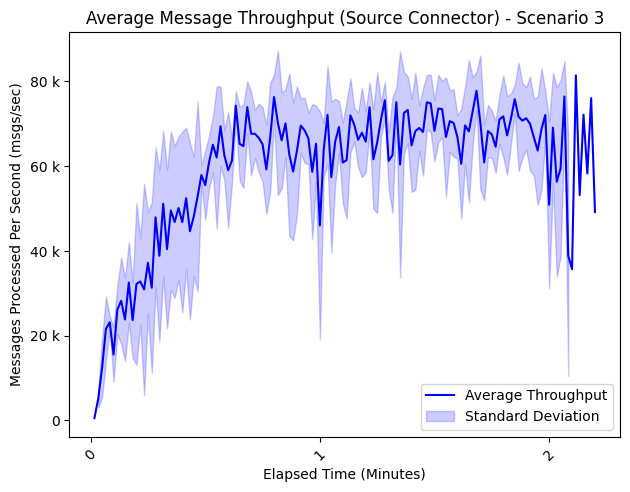
\includegraphics[width=0.5\textwidth]{chapters/images/source-performance/source-avg-messages-scenario3.png}
    }
    % \hfill
    \subfloat[Scenario 4]{\label{fig:appendix02:results:sourcemessages:scenario4}
        % \centering
        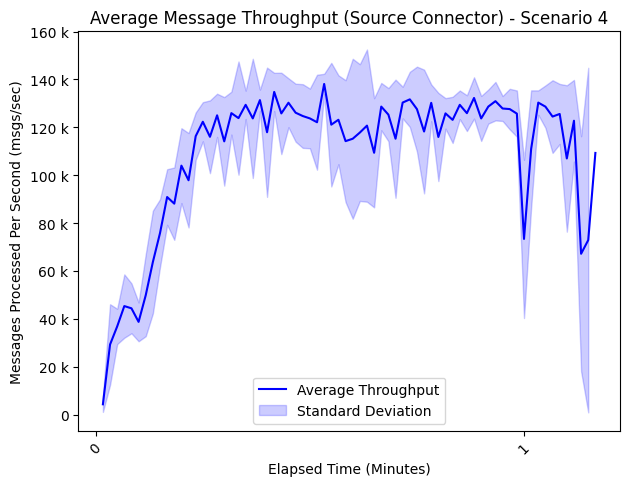
\includegraphics[width=0.5\textwidth]{chapters/images/source-performance/source-avg-messages-scenario4.png}
    }
    \hfill
    \centering
    \subfloat[Scenario 5]{\label{fig:appendix02:results:sourcemessages:scenario5}
        % \centering
        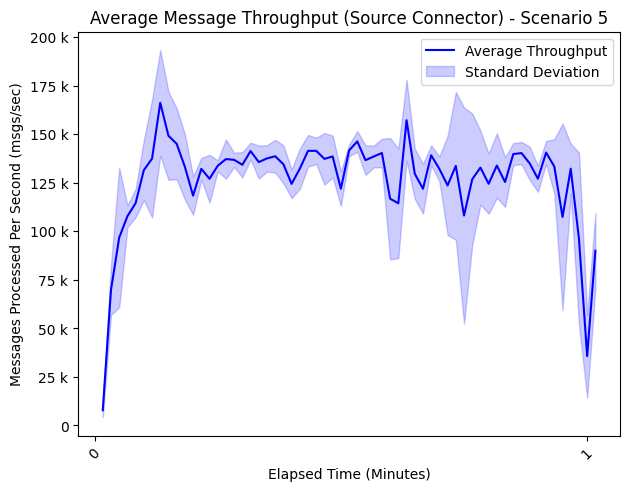
\includegraphics[width=0.5\textwidth]{chapters/images/source-performance/source-avg-messages-scenario5.png}
    }
    \hfill
    \caption{Average message throughput of various Kafka replication scenarios (source connector)}
    \label{fig:appendix02:results:sourcemessages}
\end{figure}
%%%%%%%%%%%%%%%%%%%%%%%--------TRANSACTION THROUGHPUT SOURCE--------%%%%%%%%%%%%%%%%%%%%%%%%
\begin{figure}[htbp]
    % \centering
    \subfloat[Scenario 1]{\label{fig:appendix02:results:sourcetransactions:scenario1}
        % \centering
        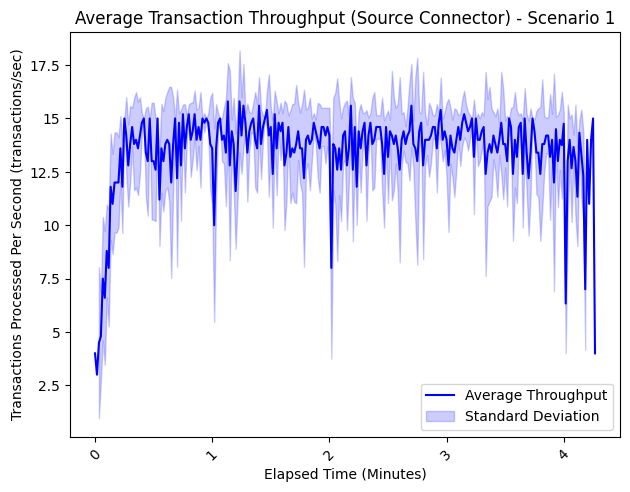
\includegraphics[width=0.5\textwidth]{chapters/images/source-performance/source-avg-transactions-scenario1.png}
    }
    % \hfill
    \subfloat[Scenario 2]{\label{fig:appendix02:results:sourcetransactions:scenario2}
        % \centering
        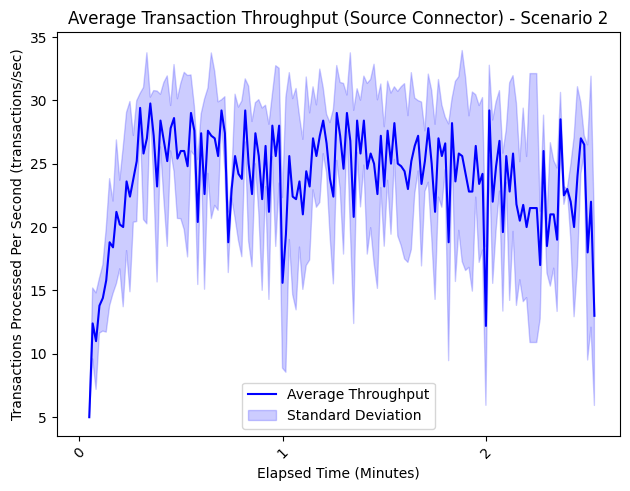
\includegraphics[width=0.5\textwidth]{chapters/images/source-performance/source-avg-transactions-scenario2.png}
    }
    \hfill
    \subfloat[Scenario 3]{\label{fig:appendix02:results:sourcetransactions:scenario3}
        % \centering
        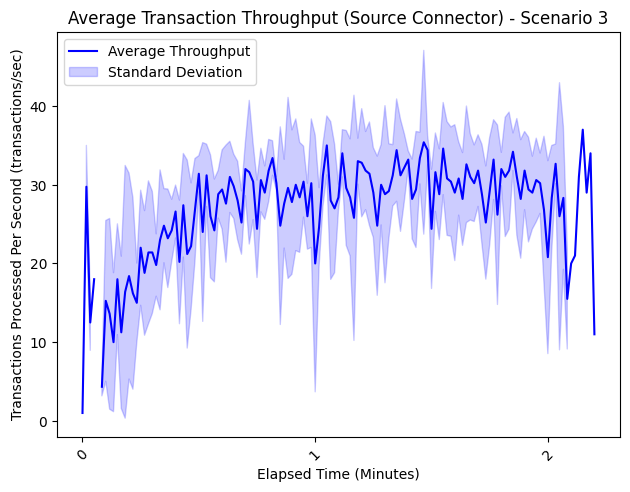
\includegraphics[width=0.5\textwidth]{chapters/images/source-performance/source-avg-transactions-scenario3.png}
    }
    % \hfill
    \subfloat[Scenario 4]{\label{fig:appendix02:results:sourcetransactions:scenario4}
        % \centering
        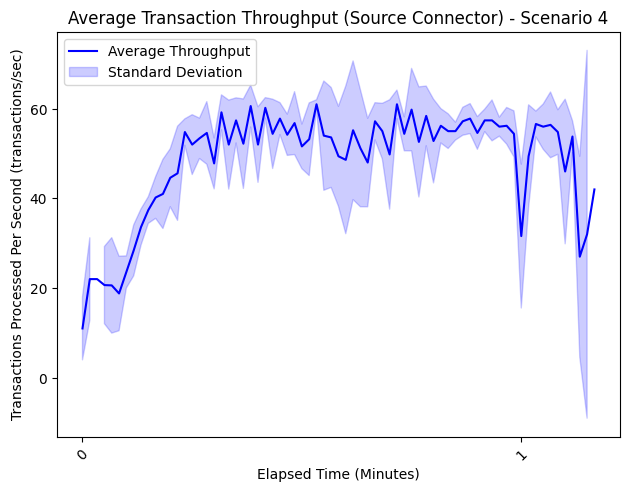
\includegraphics[width=0.5\textwidth]{chapters/images/source-performance/source-avg-transactions-scenario4.png}
    }
    \hfill
    \centering
    \subfloat[Scenario 5]{\label{fig:appendix02:results:sourcetransactions:scenario5}
        % \centering
        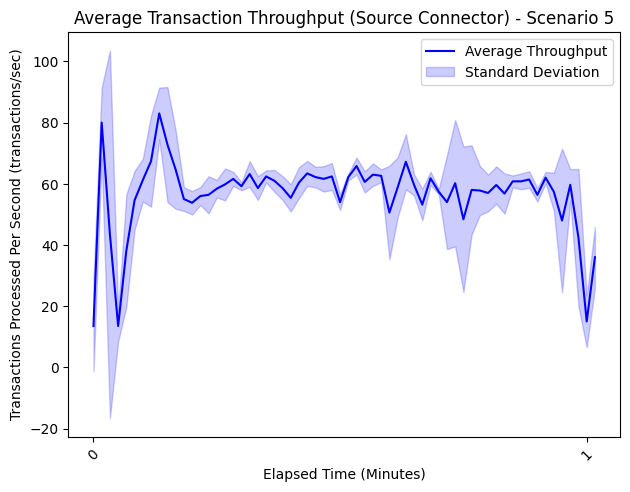
\includegraphics[width=0.5\textwidth]{chapters/images/source-performance/source-avg-transactions-scenario5.png}
    }
    \hfill
    \caption{Average transaction throughput of various Kafka replication scenarios (source connector)}
    \label{fig:appendix02:results:sourcemessages}
\end{figure}
%%%%%%%%%%%%%%%%%%%%%%%--------MESSAGE THROUGHPUT SINK--------%%%%%%%%%%%%%%%%%%%%%%%%
\begin{figure}[htbp]
    % \centering
    \subfloat[Scenario 1]{\label{fig:appendix02:results:sinkmessages:scenario1}
        % \centering
        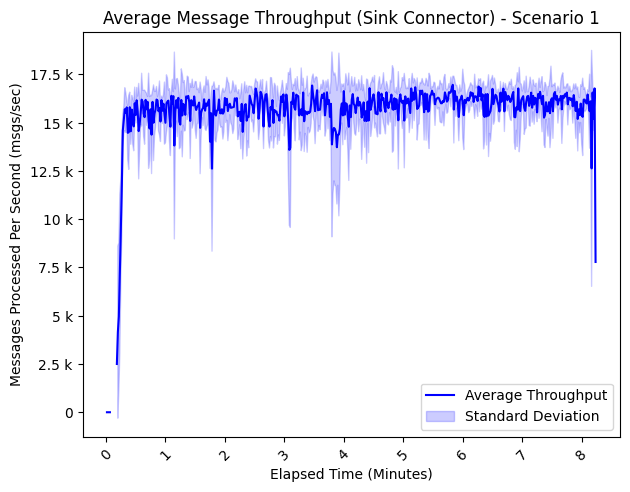
\includegraphics[width=0.5\textwidth]{chapters/images/sink-performance/sink-avg-messages-scenario1.png}
    }
    % \hfill
    \subfloat[Scenario 2]{\label{fig:appendix02:results:sinkmessages:scenario2}
        % \centering
        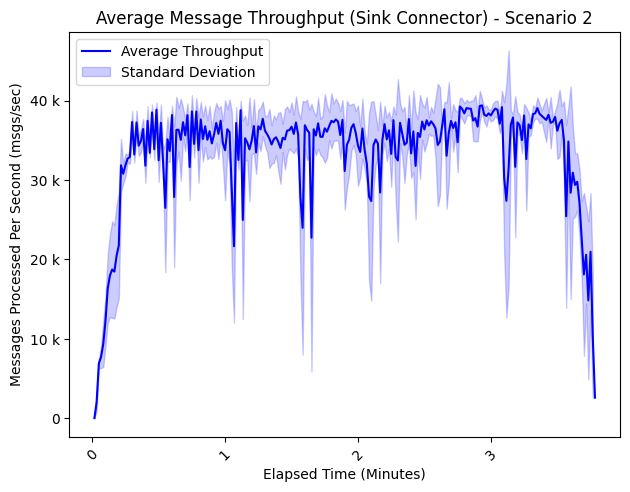
\includegraphics[width=0.5\textwidth]{chapters/images/sink-performance/sink-avg-messages-scenario2.png}
    }
    \hfill
    \subfloat[Scenario 3]{\label{fig:appendix02:results:sinkmessages:scenario3}
        % \centering
        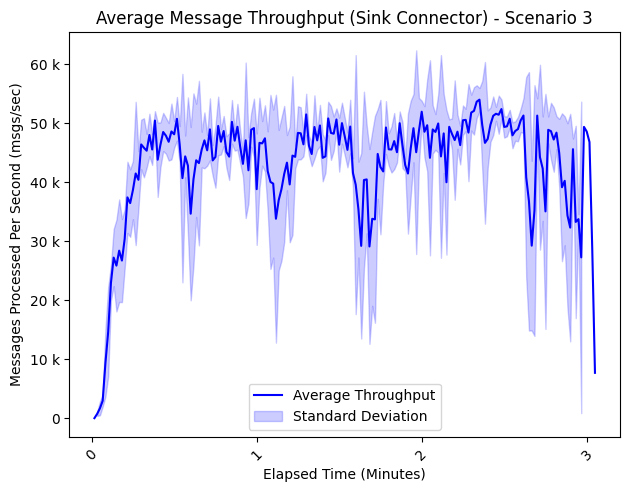
\includegraphics[width=0.5\textwidth]{chapters/images/sink-performance/sink-avg-messages-scenario3.png}
    }
    % \hfill
    \subfloat[Scenario 4]{\label{fig:appendix02:results:sinkmessages:scenario4}
        % \centering
        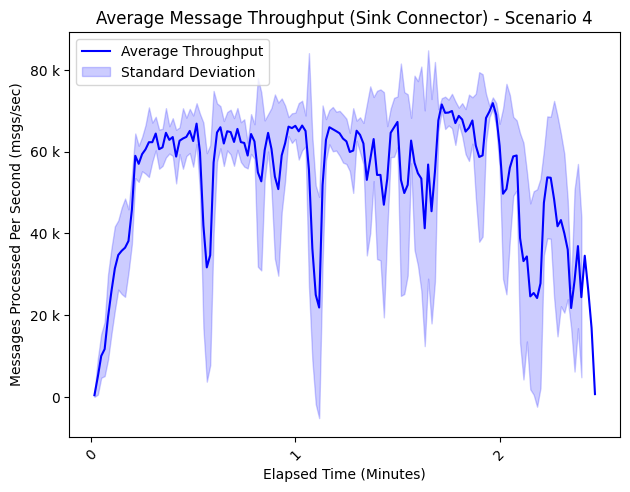
\includegraphics[width=0.5\textwidth]{chapters/images/sink-performance/sink-avg-messages-scenario4.png}
    }
    \hfill
    \centering
    \subfloat[Scenario 5]{\label{fig:appendix02:results:sinkmessages:scenario5}
        % \centering
        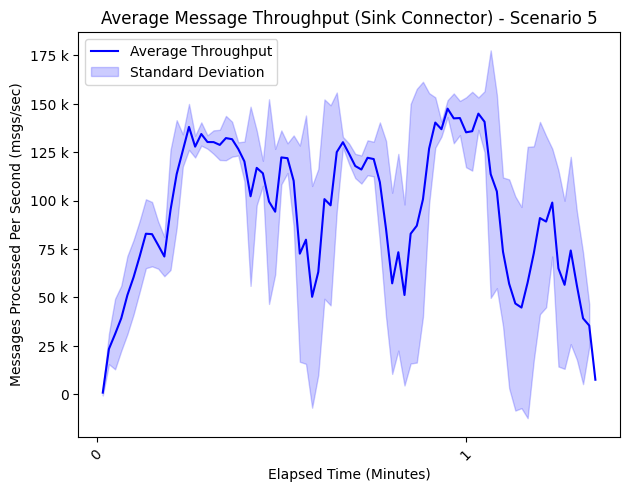
\includegraphics[width=0.5\textwidth]{chapters/images/sink-performance/sink-avg-messages-scenario5.png}
    }
    \hfill
    \caption{Average message throughput of various Kafka replication scenarios (sink connector)}
    \label{fig:appendix02:results:sinkmessages}
\end{figure}
%%%%%%%%%%%%%%%%%%%%%%%--------MESSAGE THROUGHPUT BROKER--------%%%%%%%%%%%%%%%%%%%%%%%%
\begin{figure}[htbp]
    % \centering
    \subfloat[Scenario 1]{\label{fig:appendix02:results:brokermessages:scenario1}
        % \centering
        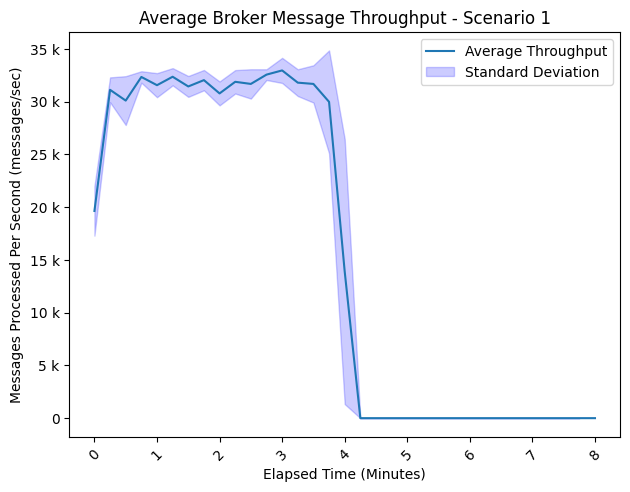
\includegraphics[width=0.5\textwidth]{chapters/images/broker-performance/broker-avg-messages-scenario1.png}
    }
    % \hfill
    \subfloat[Scenario 2]{\label{fig:appendix02:results:brokermessages:scenario2}
        % \centering
        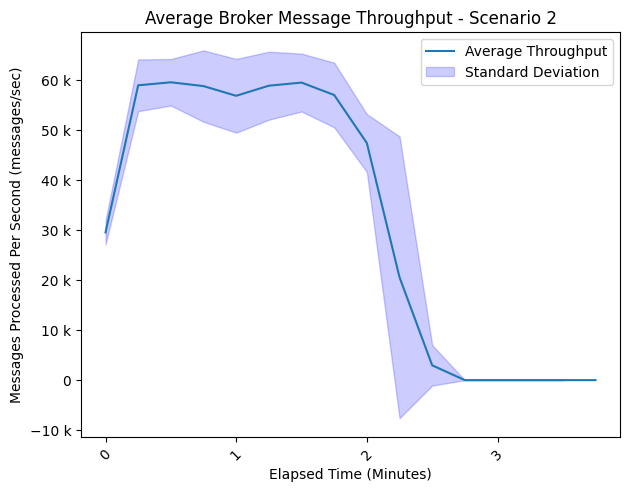
\includegraphics[width=0.5\textwidth]{chapters/images/broker-performance/broker-avg-messages-scenario2.png}
    }
    \hfill
    \subfloat[Scenario 3]{\label{fig:appendix02:results:brokermessages:scenario3}
        % \centering
        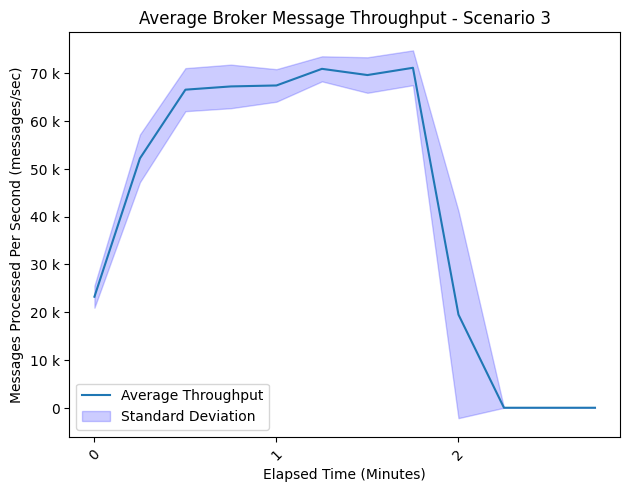
\includegraphics[width=0.5\textwidth]{chapters/images/broker-performance/broker-avg-messages-scenario3.png}
    }
    % \hfill
    \subfloat[Scenario 4]{\label{fig:appendix02:results:brokermessages:scenario4}
        % \centering
        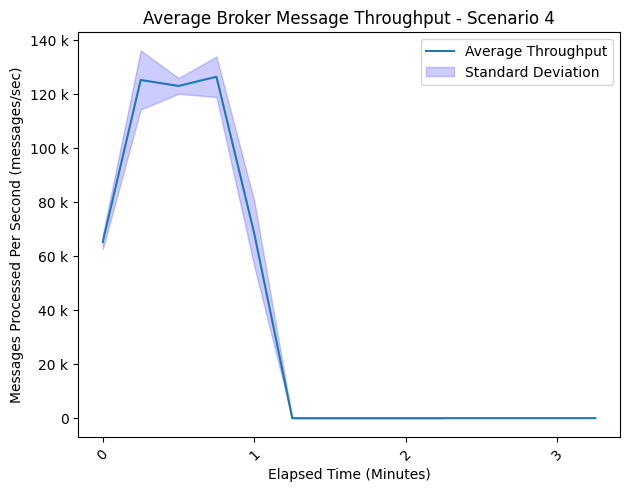
\includegraphics[width=0.5\textwidth]{chapters/images/broker-performance/broker-avg-messages-scenario4.png}
    }
    \hfill
    \centering
    \subfloat[Scenario 5]{\label{fig:appendix02:results:brokermessages:scenario5}
        % \centering
        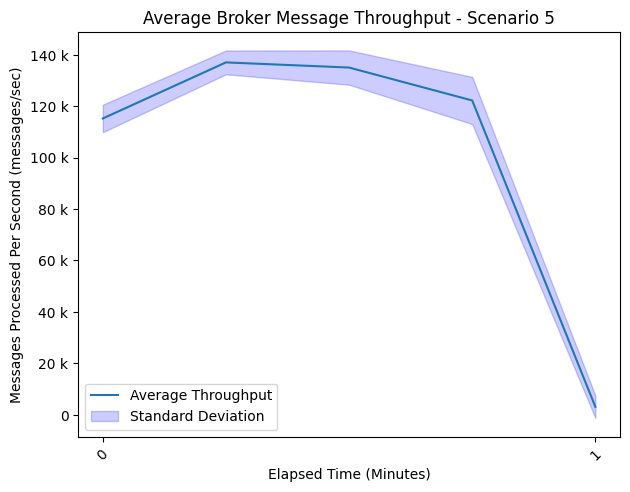
\includegraphics[width=0.5\textwidth]{chapters/images/broker-performance/broker-avg-messages-scenario5.png}
    }
    \hfill
    \caption{Average message throughput of various Kafka replication scenarios (broker)}
    \label{fig:appendix02:results:brokermessages}
\end{figure}